\section{Summary}

With two RTOS, Contiki and RIOT, and two boards, the RE-mote and the Z1, we have collected data that will define which approach best fits our framework.

With our first approach, we discovered that using the internal real-time clock to compute the context switching time is not suited for our benchmarking framework.
Moreover, outputting measurements to the serial port induce a large overhead that could prevent the benchmarked application to run correctly.

The second approach helps our framework to gather precise measurements.
With the PSLab as the external devices, the framework was able to measure precisely the context switching time on both Contiki and RIOT.

When comparing the distribution of the two approaches to the real context switching time distribution, it is clear that the devices approach is the best fit for our benchmarking framework.

The figure \ref{fig:comparison-all-contiki-remote} and the figure \ref{fig:comparison-all-contiki-z1} show the comparison between the first and the second approach on the RE-mote and the Z1 boards with Contiki.
With a large distribution, it is difficult to see the difference between the reference distribution and the devices approach measurements distribution.
However, we can see that the distribution of the extension approach measurements does not match the distribution of our reference measurements.

\begin{figure}[!ht]
  \centering
  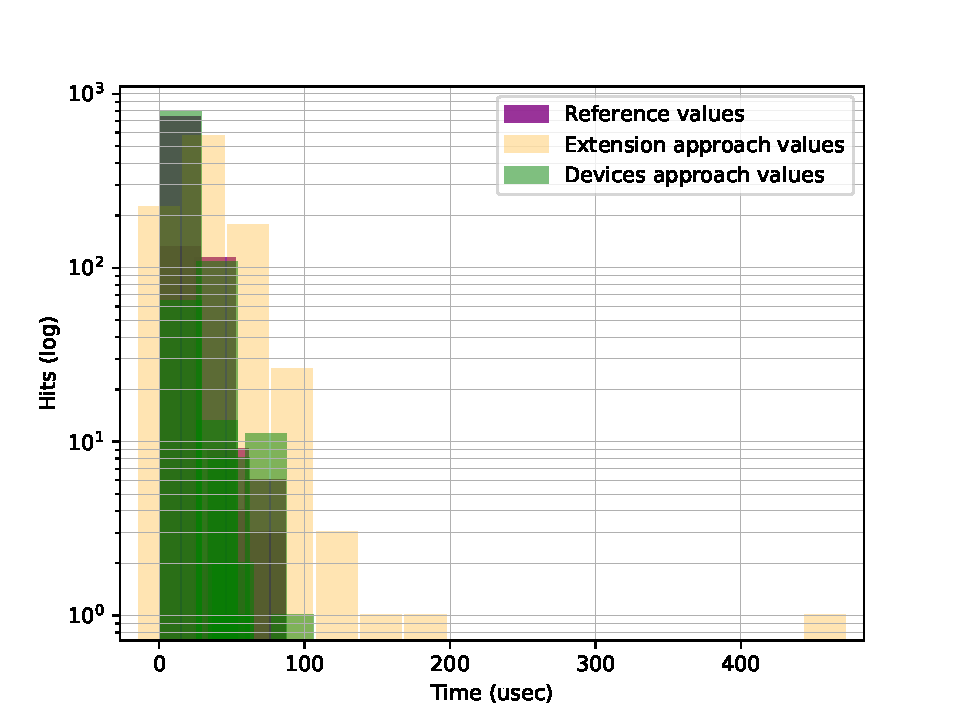
\includegraphics[scale=.7]{assets/comparison-all-contiki-remote.pdf}
  \caption{comparison of the two approaches with Contiki on the RE-Mote board\label{fig:comparison-all-contiki-remote}}
\end{figure}

\begin{figure}[!ht]
  \centering
  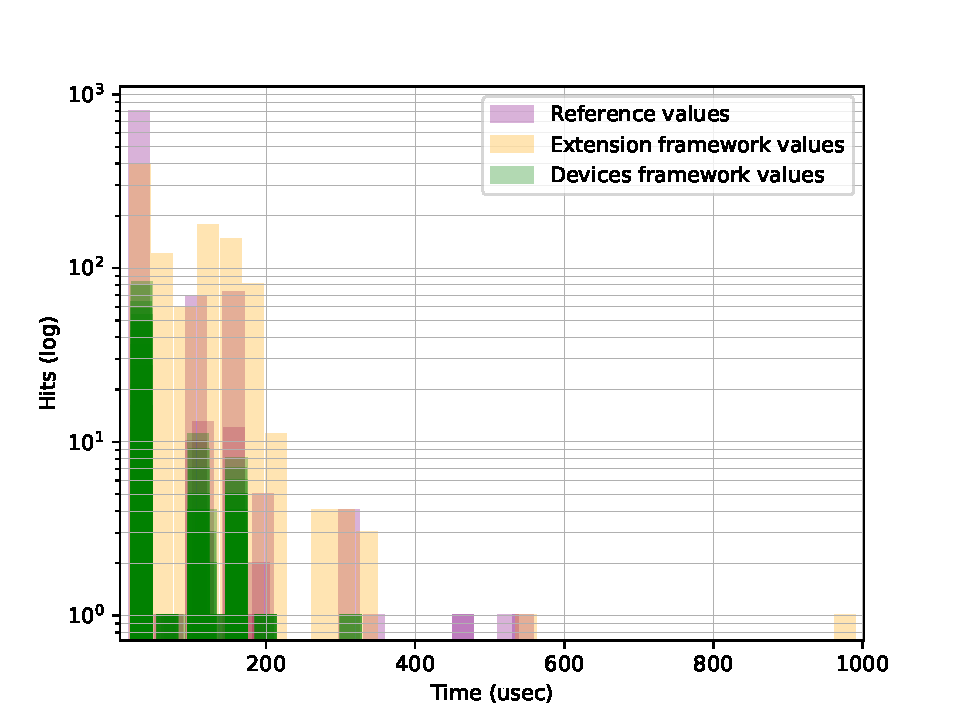
\includegraphics[scale=.7]{assets/comparison-all-contiki-z1.pdf}
  \caption{comparison of the two approaches with Contiki on the Z1 board\label{fig:comparison-all-contiki-z1}}
\end{figure}

The figure \ref{fig:comparison-all-riot-remote} and the figure \ref{fig:comparison-all-riot-z1} show the comparison between the first and the second approach on the RE-mote and the Z1 boards with RIOT.
The devices approach is the closest to the reference measurements.
As the distribution measurements is narrower with RIOT than with Contiki, the difference is more visible.

\begin{figure}[!ht]
  \centering
  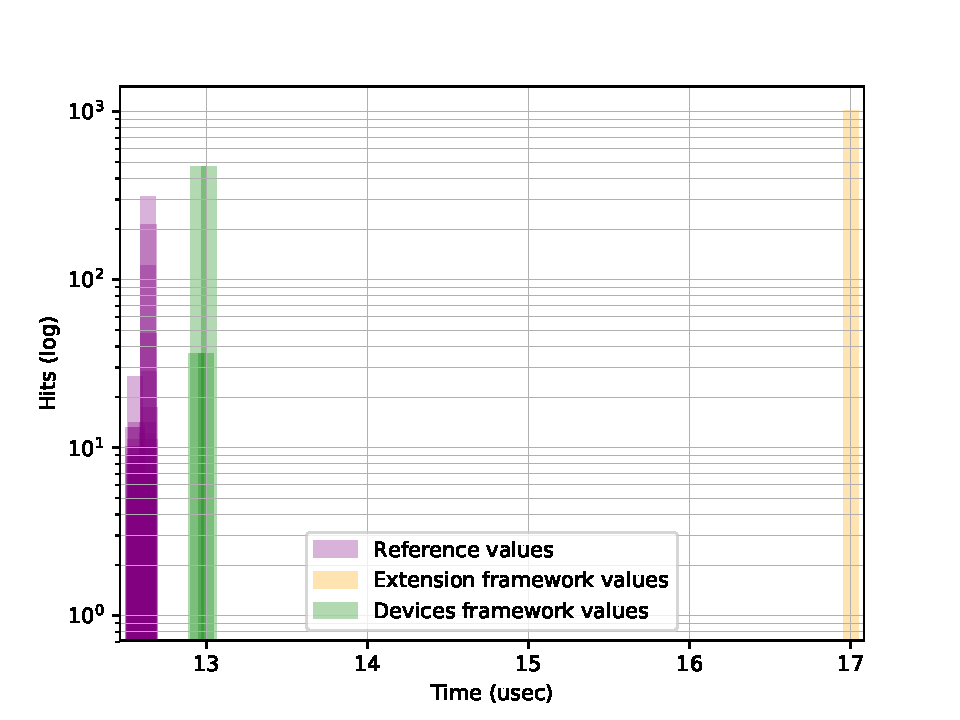
\includegraphics[scale=.7]{assets/comparison-all-riot-remote.pdf}
  \caption{comparison of the two approaches with RIOT on the RE-Mote board\label{fig:comparison-all-riot-remote}}
\end{figure}

\begin{figure}[!ht]
  \centering
  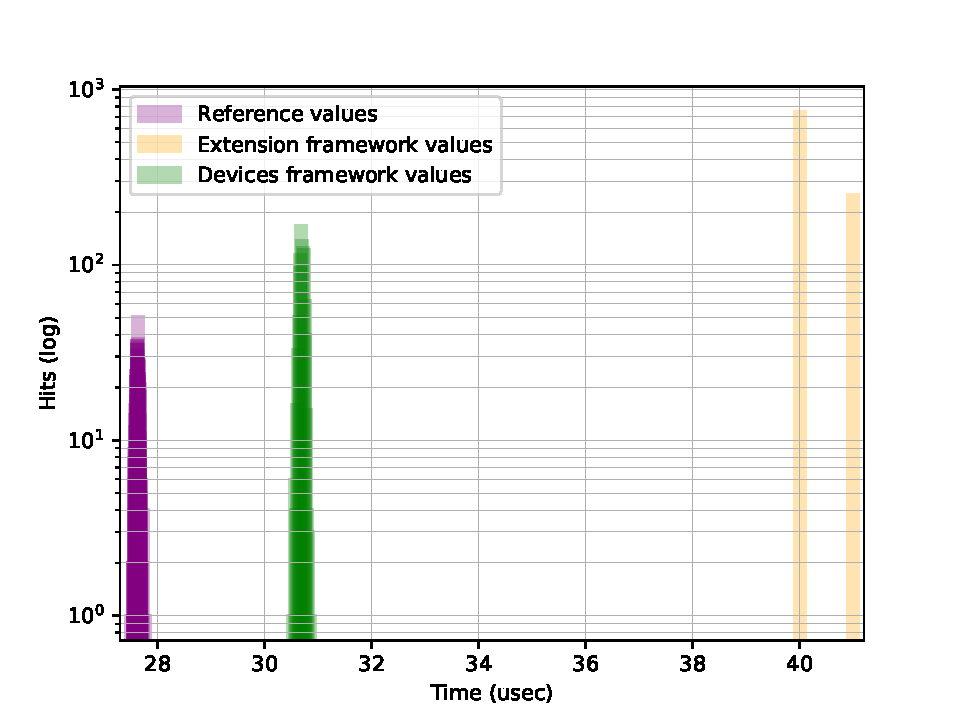
\includegraphics[scale=.7]{assets/comparison-all-riot-z1.pdf}
  \caption{comparison of the two approaches with RIOT on the Z1 board}\label{fig:comparison-all-riot-z1}
\end{figure}